\documentclass[../thesis.tex]{subfiles}
\begin{document}

\chapter{validation}
\label{chp:validation}

Within this chapter the model validation is explained and described. At first the experimental setup used in the performed experiments is shown and then the experimental and model results are explained. After that a comparison is done to show that the model is performing as expected.

\section{experimental setup}

The experiments used for validating the developed model where done using a sounding rocket as part of the \texttt{MORABA} (\textbf{Mo}bile \textbf{Ra}cketen \textbf{Ba}sis) \cite{stamminger2012moraba} setup. The mission's name was \texttt{TEXUS-57}. The experimental setup as shown in \cite{stergiou2022effects} is visible in \autoref{fig: experiment}.
\begin{figure}[htbp]
	\centering
	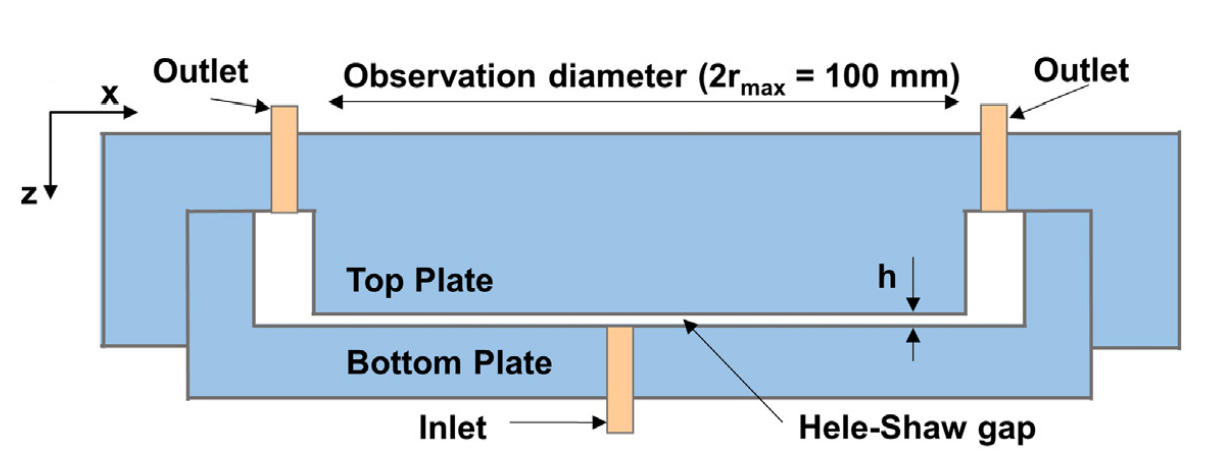
\includegraphics[scale=0.4]{experimental_setup}
	\caption{experimental setup for validation}
	\label{fig: experiment}
\end{figure}
The gap height $h$ used for the experiments was 0.2 mm. The experiment is observed by a camera from the top throughout the hole run. These gained images are the base for further analysis.

\section{experimental results}

An image example as gained by the experiments is shown in \autoref{fig: exp_img}. The analysis on this images is done using image processing. The image is converted to a gray-scale image as a first step. Then the gained values are correlated to concentration values using the known values for the input's concentrations. Based on the gained product concentration values the reaction front's front and back positions are gained by a threshold operation. The position of the fronts maximum is computed by detecting the position of the maximum gray value within the image. The results are stored within \texttt{.csv} files. The file containing the fronts position has the form shown in \autoref{tab: front_csv}. 

\begin{table} [htb]
	\centering
	\caption{front position output format}
	\begin{tabular}{ cccc }
		\hline
		t (s) & WC (mm) & RC (mm) & Rf (mm) \\
		\hline
		46.333 & 2.4949 & 5.6819 & 8.1854 \\
		... & ... & ... & ... \\
		52 & 3.0455 & 6.2054 & 8.7207 \\
		... & ... & ... & ... \\
		\hline
		\label{tab: front_csv}
	\end{tabular}
\end{table}
t describes the flow time during the experiment in seconds and WC is front's width. The width is calculated using the difference between the front's front and back positions. RC is the radial distance from the center of the front's maximum and Rf is the front's front position.
In addition to the front's positions the total amount of product formed is calculated. This is done by integrating the concentration values over the hole domain and gap height. To make experiments more easily comparable with each other the formed product values (in mol) are non-dimensionalized. To achieve this the values are divided by $c_{max} \cdot V_{reactor}$. The variable $c_{max}$ is the maximum value of the product's concentration during one experimental run and $V_{reactor}$ is the reactor's volume. The product of these two values refers to the fully mixed case as it gives in indication of the maximum amount of product possible than can be created. The format of the results is shown in \autoref{tab: product_csv}. The volume injected is equivalent to the time elapsed in seconds. These two values can be converted using the flow rate. NC is the non-dimensional product formed for each time step.

\begin{table} [htb]
	\centering
	\caption{product formed output format}
	\begin{tabular}{ cc }
		\hline
		Volume injected (mL) & NC (-) \\
		\hline
		0 & 0.011312 \\
		... & ... \\
		0.01072 & 0.011907 \\
		... & ... \\
		\hline
		\label{tab: product_csv}
	\end{tabular}
\end{table}

\section{model results}
\label{sec: model res}

The results gained from the model are no images but tables with all exported values. These tables are created at each interval defined by the user as shown in \autoref{}.

\section{comparison}

For comparison the position of the product's maximum is used.

\end{document}